%MQ_list_isomorphisms

\documentclass[problem]{mcs}

\begin{pcomments}
\pcomment{MQ_planar_graph_properties}
\end{pcomments}

\pkeywords{
  planar_graphs
  planar_embeddings
  discrete_face
  face
  graph_coloring
  colorable
}

%%%%%%%%%%%%%%%%%%%%%%%%%%%%%%%%%%%%%%%%%%%%%%%%%%%%%%%%%%%%%%%%%%%%%
% Problem starts here
%%%%%%%%%%%%%%%%%%%%%%%%%%%%%%%%%%%%%%%%%%%%%%%%%%%%%%%%%%%%%%%%%%%%%

\begin{problem}
  Remember this awesome graph from last miniquiz? Let's solve some more fun problems about it!

\begin{center}
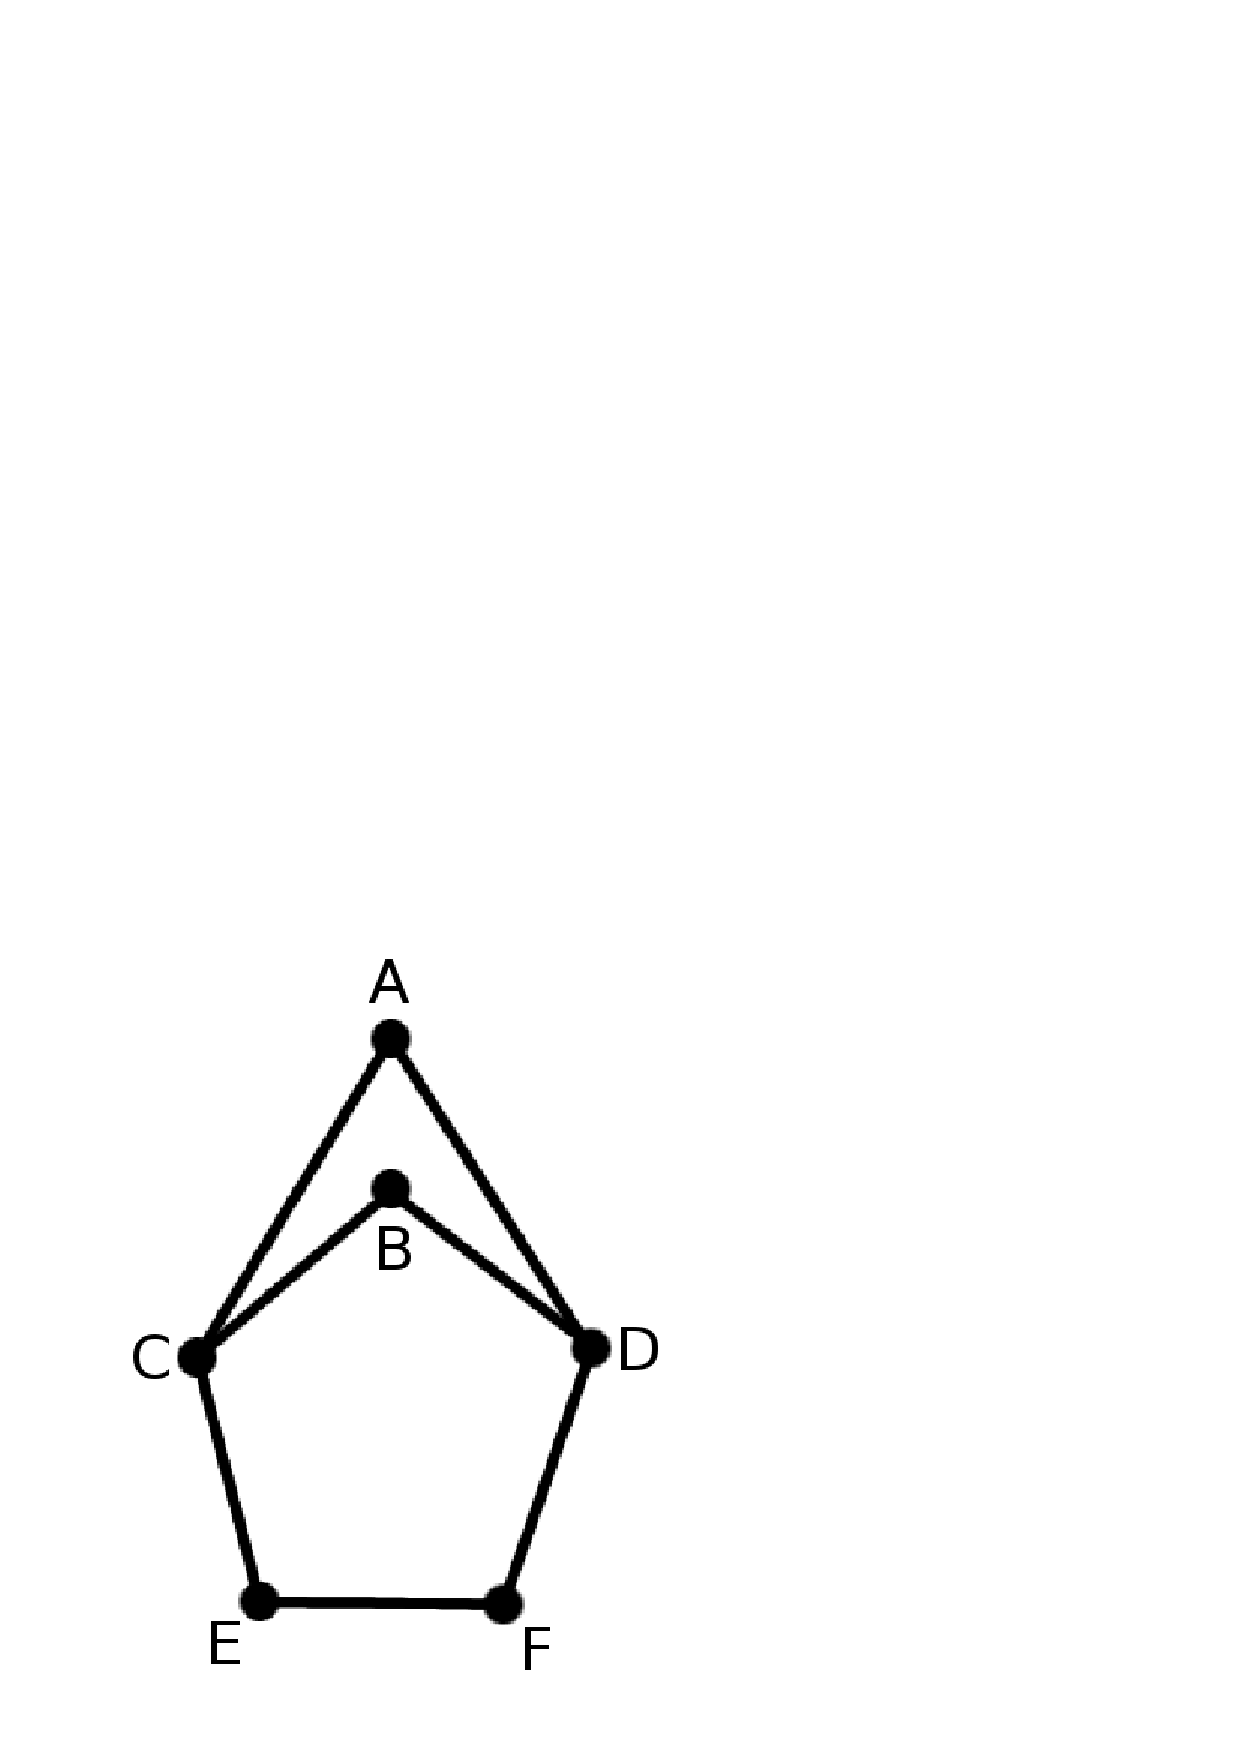
\includegraphics[height=2in]{figures/planar_graph_morning.pdf}
\end{center}

\bparts

\ppart What is its chromatic number? \brule{0.4in}

\ppart Notice that it's a connected planar graph. Describe all of its discrete faces.

\eparts

\begin{solution}
TBA
\end{solution}

\end{problem}

%%%%%%%%%%%%%%%%%%%%%%%%%%%%%%%%%%%%%%%%%%%%%%%%%%%%%%%%%%%%%%%%%%%%%
% Problem ends here
%%%%%%%%%%%%%%%%%%%%%%%%%%%%%%%%%%%%%%%%%%%%%%%%%%%%%%%%%%%%%%%%%%%%%

\endinput
